%% ****** ljmsamp.tex 13.06.2018 ******
\documentclass[11pt, tightenlines, twoside, onecolumn, nofloats, nobibnotes, nofootinbib, superscriptaddress, noshowpacks, centertags]{revtex4}
\usepackage{ljm}

\usepackage[ruled,vlined]{algorithm2e}
\usepackage{tikz}
\usetikzlibrary{positioning}


\begin{document}
\newcommand{\ls}{[}
\newcommand{\rs}{]}
\newcommand{\lp}{\big(}
\newcommand{\rp}{\big)}
\renewcommand{\bold}{\mathbf}
\theoremstyle{remark}

\newtheorem*{remark}{Remark}
\newtheorem{claim}{Claim}

\titlerunning{Predicting optimal superposition trees in symbolic regression}
\authorrunning{R.\,G.~Neychev,  I.\,A.~Shibaev, V.\,V.~Strijov}
\title{Predicting optimal superposition trees in symbolic regression}

\author{\firstname{R.\,G.}~\surname{Neychev}}
\email[E-mail: ]{neychev@phystech.edu}
\affiliation{Moscow Institute of Physics and Technology, 9 Institutskiy per., Dolgoprudny, 141701, Russia}

\author{\firstname{I.\,A.}~\surname{Shibaev}}
\email[E-mail: ]{shibaev.kesha@gmail.com}
\affiliation{Moscow Institute of Physics and Technology, 9 Institutskiy per., Dolgoprudny, 141701, Russia}
%\affiliation{Example: N.I. Lobachevskii Institute of Mathematics and Mechanics, Kazan (Volga Region) Federal University, Kremlevskaya ul. 18, Kazan, Tatarstan, 420008 Russia}

\author{\firstname{V.\,V.}~\surname{Strijov}}
\email[E-mail: ]{strijov@phystech.edu}
\affiliation{Moscow Institute of Physics and Technology, 9 Institutskiy per., Dolgoprudny, 141701, Russia}
\affiliation{Dorodnitsyn Computing Centre FRC CSC RAS, 40 Vavilova., 119333, Russia}

%\firstcollaboration{(Submitted by A.~A.~Editor-name)} % Add if you know submitter.
%\lastcollaboration{ }

\received{December 02, 2020} % The date of receipt to the editor, i.e. December 06, 2017


\begin{abstract} % You shouldn't use formulas and citations in the abstract.
This paper investigates the problem of regression model  generation. A model is a superposition of primitive functions. The model structure is described by a weighted colored graph. A graph node corresponds to some primitive function. An edge sets a superposition of two functions. The weight of an edge sets a probability of the superposition. To generate an optimal model one  has to reconstruct its structure from an adjacency matrix. This matrix contains superposition probabilities. The presented solution is based on search of minimum spanning tree in weighted colored graph. Solutions to symbolic regression problems tend to be easier to interpret and more effective. The symbolic regression problem is solved via restoration of the superposition tree from the predicted adjacency matrix. The restoration procedure is sensitive to noise in the predicted matrix. This paper presents a novel approach based on Prize-Collecting Steiner Tree algorithm. The proposed algorithm is compared with existing approaches to superposition trees restoration from noised adjacency matrix. Synthetic data is used in the experimental setup.
\end{abstract}

\subclass{15A09, 15A63, 62J05, 62H30, 62H86} % Enter 2010 Mathematics Subject Classification.

\keywords{forecasting model, symbolic regression, superposition, minimum spanning tree, adjacency matrix} % Include keywords separated by comma.

\maketitle

% Text of article starts here.

\section{Introduction}
Symbolic regression is a well known approach to regression problems. It aims the optimization of the selected criteria with superposition of functions from some basis set. Such approach delivers simple yet accurate solutions. The derived solutions are much easier to interpret compared to deep neural networks or tree ensembles, which is a necessary property in many domains, especially in medicine or fraud-detection.

Symbolic regression problems usually require complex computations. While different approaches are used to find the optimal subset of the basis functions set, genetic algorithms~\cite{davis1991handbook} are one of the most popular ones. The symbolic regression problem is a popular illustration of the genetic programming~\cite{koza1994genetic}. More specific approaches are used if additional constraints are present (e.g. linear combinations of basis functions~\cite{searson2010gptips,searson2015gptips} only).
The symbolic regression might be considered as structural optimization problem, widely known in Deep Learning. Recent achievements show the promising outlook of the genetic algorithms~\cite{evolving2002,wann2019}.

Different approach to solving the symbolic regression problems is based on matrix representation~\cite{Bochkarev2017} of the computation graph of the target function. This leads to the necessity of superposition matrix prediction. However, fuzzy classification methods do not consider the constraints of the arity of used functions and the tree orientation. Solutions based on the classification methods predictions of the adjacency matrix are rather unstable solutions, the computational graph contains many low-probability edges.

This paper approaches the symbolic regression problem restoring the superposition matrix from the predicted edge probabilities. The solution incorporates several steps. First, the original problem is reduced to the $k$-minimum spanning tree ($k$-MST) problem. This problem is NP-hard~\cite{lozovanu1993minimal}, so only approximate solutions are applicable~\cite{ravi1996spanning}. The $k$-MST problem can be approached as Prize-Collecting Steiner Tree (PCST) problem~\cite{Chudak2004} due to the equivalency of the relaxed formulations of the Linear Programming problem statements.

Many approximate solutions are present for the $k$-MST problem~\cite{ravi1996spanning,awerbuch1998new,Arora2006}. The approach presented in~\cite{Arora2006} is based on the classic PCST problem solution with $(2-\varepsilon)$ factor, which is described in~\cite{goemans1995general}. In case of known root node the undirected tree can be restored to the directed one. Hence the algorithm restoring undirected tree from the graph in PCST problem might be used. Then the superposition matrix is restored from the directed tree.

This paper proposes a novel approach to solving the symbolic regression problem by restoring the superposition tree. The proposed solution is based on the relaxed version of $k$-MST problem, which transforms to PCST problem with constant prizes same for all vertices. The fast algorithm for PSCT problem is described in~\cite{hegde2014fast}, source code available in~\cite{pcstfast_alg}. The proposed approach is based on $(2-\varepsilon)$ approximating algorithm for PSCT problem. This approach is compared with variety of other solutions based on DFS and BFS and Prim's algorithm using the synthetic data.

\section{Problem statement}

There given a collection of datasets $\mathcal{A}=\{\bold A_1,\ldots,\bold A_N\}$. Every dataset $\bold A_i=(\bold X_i,\bold y_i)$ the object matrix $\bold X_i$ and the target values vector $\bold y_i$ of length $n_i$. Denote a function $f_i$ such that $f_i(\bold X_i) = y_i$. This function is a superposition of basic functions $g_1,\ldots,g_l$. Let's call $f_i$ a \emph{generative} superposition for the dataset $\bold A_i$.

All the datasets in the collection $\mathcal{A}$ are \emph{homogeneous} w.r.t. the family of generative superpositions $\mathcal{F}$, where $\mathcal{F}=\{f:f=\sup(g_1,\ldots,g_l)\},$  $f_i\in\mathcal{F} \forall i$. 

The optimal superposition $f^{\ast}$ for every fixed pair $\bold A= (\bold X,\bold y)$ is derived from the following optimization problem:
\begin{align}
f^{\ast} = \arg\min\limits_{f\in \mathcal{F}}S(f|\bold X,\bold y),
\label{task_1}
\end{align}
where $S$ stays for the \emph{loss function}. In the following paper Squared Deviation is used for this purpose:
\[S(f|\bold X,\bold y)= \| f(\bold X)-\bold y\|_2^2.\]

\subsection{The proposed solution}

Denote the mapping $h:\mathcal{A}\to\mathcal{F}$ which delivers the solution for the problem~(\ref{task_1}). The optimization problem takes the following interim form:
\begin{align*}
h^{\ast}=\arg\min\limits_{h\in H}\sum_{i=1}^{N}\| h(\bold A_i)(\bold X_i)-\bold y_i\|_2^2,
\end{align*}
where $H$ is some parametric set of potential mappings. Due to the original problem formulation, every dataset $\bold A_i$ is paired with the \emph{generative} superposition $f_i$, such that $\| f_i(\bold X_i)-\bold y_i\|_2=0$ (while its original form may be unknown). The optimization problem then takes the final form:
\begin{align}
h^{\ast}=\arg\min\limits_{h\in H}\sum_{i=1}^{N}\|\left( h(\bold A_i)-f_i\right)(\bold X_i)\|_2^2,
\label{task_2}
\end{align}
so the optimal mapping $h(A_i)$ delivers the optimal approximation of the superposition $f_i$ in closed form.


Every superposition $f_i$ can be represented as a graph where the basic functions are placed in the nodes. The similar representation is proposed in~\cite{Bochkarev2017}. This approach is illustrated with the following example.

\begin{minipage}[B]{0.25\textwidth}
    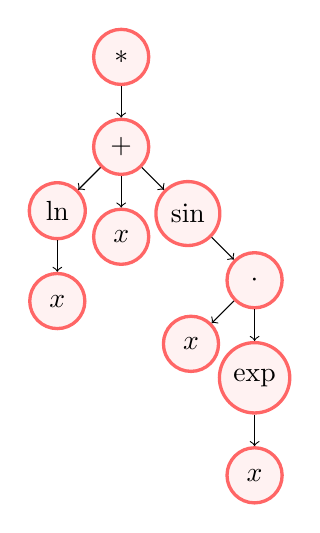
\begin{tikzpicture}[
        roundnode/.style={circle, draw=red!60, fill=red!5, very thick, minimum size=7mm},
        node distance=0.4cm
        ]
        \node[roundnode]            (q_0)                           {$\ast$};
        \node[roundnode]                    (q_1) [below         =of q_0]     {$+$};
        \node[roundnode]                    (q_2) [below left    =of q_1]     {$\ln$};
        \node[roundnode]                    (q_3) [below         =of q_1]     {$x$};
        \node[roundnode]                    (q_4) [below right   =of q_1]     {$\sin$};
        \node[roundnode]                    (q_5) [below         =of q_2]     {$x$};
        \node[roundnode]                    (q_6) [below right   =of q_4]     {$\cdot$};
        \node[roundnode]                    (q_7) [below left    =of q_6]     {$x$};
        \node[roundnode]                    (q_8) [below         =of q_6]     {$\exp$};
        \node[roundnode]                    (q_9) [below         =of q_8]     {$x$};
        \path[->]
        (q_0)   edge                    node    {}  (q_1)
        (q_1)   edge                    node    {}  (q_2)
        edge                    node    {}  (q_3)
        edge                    node    {}  (q_4)
        (q_2)   edge                    node    {}  (q_5)
        (q_4)   edge                    node    {}  (q_6)
        (q_6)   edge                    node    {}  (q_7)
        edge                    node    {}  (q_8)
        (q_8)   edge                    node    {}  (q_9);
    \end{tikzpicture}
    \captionof{figure}{Computational graph}
    \label{graph}
\end{minipage}
\begin{minipage}[B]{0.35\textwidth}
    \centering
        \begin{tabular}{|c|c||c|c|c|c|c|c|c|}
                \hline
                ar&$f(.)$&$\ast$&$+$&$\ln$&$\sin$&$\cdot$&$\exp$&x\\
                \hline
                $1$&$\ast$ &0&1&0&0&0&0&0\\
                \hline
                $3$&$+$    &0&0&1&1&0&0&1\\
                \hline
                $1$&$\ln$  &0&0&0&0&0&0&1\\
                \hline
                $1$&$\sin$ &0&0&0&0&1&0&0\\
                \hline
                $2$&$\cdot$&0&0&0&0&0&1&1\\
                \hline
                $1$&$\exp$ &0&0&0&0&0&0&1\\
                \hline
        \end{tabular}
    \captionof{table}{Adjacency matrix}
    \label{adjacency_matrix}
\end{minipage}
\begin{minipage}[B]{0.35\textwidth}
    \centering
        \begin{tabular}{|c|c||c|c|c|c|c|c|c|}
            \hline
            ar&$f(.)$&$\ast$&$+$&$\ln$&$\sin$&$\cdot$&$\exp$&x\\
            \hline
            $1$&$\ast$ &0.2&0.7&0.5&0.4&0.5&0.3&0.2\\
            \hline
            $3$&$+$    &0.3&0.2&1.&0.8&0.6&0.3&0.7\\
            \hline
            $1$&$\ln$  &0.3&0.2&0&0.&0.1&0.5&0.5\\
            \hline
            $1$&$\sin$ &0.1&0.4&0&0.5&0.9&0.2&0.5\\
            \hline
            $2$&$\cdot$&0.3&0.&0.3&0.5&0.&0.8&0.6\\
            \hline
            $1$&$\exp$ &0.3&0.3&0.4&0.1&0.5&0.4&0.4\\
            \hline
        \end{tabular}
    \captionof{table}{Probability of adjacency matrix}
    \label{restored_adjacency_matrix}
\end{minipage}

Denote function $f(x) = \ln(x) + x + \sin(x\cdot e^x)$. Its graph form is shown on figure \ref{graph} and corresponding adjacency matrix is provided in table \ref{adjacency_matrix}. The \emph{root} node is represented with the wildcard $\ast$ symbol. Node $x$ is repeated only for the visual sake.

To reconstruct the original function $f$ one need only the graph visualization (or the corresponding adjacency matrix) and the mapping between the nodes indices and basic functions.

Hereinafter all the superpositions are constructed with the following procedure:
\begin{itemize}
\item The set basic functions (with fixed arity) $g$ is defined and extended with the special function $\ast=\ast(x):\ast(x)=x$ for the \emph{root} node.
    \item The graph is constructed with the basic functions as the nodes. The directed tree is defined with this graph, where the \emph{root} node is represented with $\ast$.
    % \item Every edge $e_{ij}$ between nodes $i$ and $j$  $\ldots$
\end{itemize}

\subsubsection{Symbolic Regression Problem Statement in matrix form}

Problem~(\ref{task_2}) can be reformulated in the matrix form:
\begin{align*}
h^{\ast}=\arg\min\limits_{h\in H}\sum_{i=1}^{N}\|\left(F(M(h(\bold A_i)))-F(M(f_i))\right)(\bold X_i)\|_2^2,
\end{align*}
where $M$ maps function $f$ to matrix form $m$ and $F$ maps matrix form $m$ to function $f$.

Small deviations in the superposition matrix cause significant changes in the restored function. The following formulation focuses on finding the correct superposition matrix:

\begin{align*}
h^{\ast}=\arg\max\limits_{h\in H}\sum_{i=1}^{N}\ls M(h(\bold A_i))=M(f_i)\rs.
\end{align*}

The final mapping $h:\mathcal{A}\to\mathcal{F}$ incorporates several steps: $h(A_i) = F(R(P(A_i)))$. 
\begin{itemize}
    \item The mapping $P:\bold X\times \bold y\to \bold M$ (P stands for "predict") maps the original data points combined with labels $(\bold X, \bold y)$ to approximate superposition matrices $M=P(\bold A)$. All elements of the matrix have the following property: $M_{ij}\in[0, 1]$.
    \item The mapping $R: M\to M$ (R stands for "restore") provides the correct (in terms of \emph{arity}) superposition matrix.
    \item The mapping $F$ is already described.
\end{itemize}

Hence, the final solution can be derived from the optimization problem in the following form:
\begin{align}
h^{\ast}=\arg\max\limits_{R, P}\sum_{i=1}^{N}\ls R(P(\bold A_i))=M(f_i)\rs.
\label{task_final}
\end{align}

\subsection{Restoring the superposition tree}

\begin{definition}{Superposition tree restoration problem}
Denote the directed weighted graph $G=(V,E)$ with colored vertices $v_i$ and special vertex $r$. Every edge $e_i\in E$ $e_i$ is assigned with a weight $w(e_i)=c_i\in[0,1]$, every vertex $v_i \in V$ is assigned with a color  $t(v_i)=t_i\in\mathbb{N}$.

The goal is to construct a minimum-weight directed tree with root node $r$ covering at least $k$ vertices in this graph so that the half-step of the vertex's output $v_i$ (the number of edges coming from it) after covering is less than or equal to $t_i$ (root vertex $r$ has $t_r=1$).
\end{definition}
This constraints can be translated to the form of a linear programming problem with integer constraints:
\begin{align}
\underset{\substack{x_e,z_S \\ e\in E, S\subseteq V\backslash \{r\}}}{\text{minimize}}\quad & \sum\limits_{e\in E}c_ex_e \nonumber\\
\text{s.t.\quad} & \sum\limits_{\substack{e\in\delta(S):\\e=(\ast,v_i),~ v_i\in\delta(S)}}x_e + \sum\limits_{T:T\supseteq S}z_T\geqslant 1, & \forall S\subseteq V\backslash \{r\},\nonumber\\
& \sum\limits_{e\in E:~e=(\ast,v)}x_e\leqslant 1, & \forall v\in V,
\label{ilp_our}\\
& \sum\limits_{e\in E:~e=(v,\ast)}x_e\leqslant t_i, & \forall v\in V,\nonumber\\
& \sum\limits_{S\subseteq V\backslash \{r\}}|S|z_S \leqslant n-k,\nonumber\\
& x_e\in\{0,1\}, &\forall e\in E,\nonumber\\
& z_S\in\{0,1\}, & S\subseteq V\backslash \{r\},\nonumber
\end{align}
where $x_e = 1$ if edge $e$ is included into the final superposition and $x_e = 0$ otherwise; $z_S = 1$ for all vertices excluded from final superposition. If edge source vertex is irrelevant it is denoted as $e=(\ast, v)$; if terminal vertex is irrelevant edge is denoted as $e=(v, \ast)$.

The constraints can be treated as following:
\begin{itemize}
    \item First constraint defines the structure of the final solution as the tree with root $r$.
    \item Second constraint fixes the orientation of the final tree (so every vertex has the only incoming edge).
    \item Third constraint fixes the arity of the used basic functions (or the number of edges which has the certain vertex as their source).
    \item Fourth constraint states that the final tree has at least $k$ vertices.
\end{itemize}

\emph{If all weights are non-negative, the fourth constraint on the minimal number of vertices can take more strict form "number of vertices should be exactly $k$". However, the softer constrain allows to find possible connections with other optimization problems. The exact form of the constraints in \ref{ilp_our} has the same goal.}


\section{$\text{PCST}$ algorithm for superposition matrix restoration}
\subsection{$k\text{-MST}$ and  $\text{PCST}$ algorithms}

\begin{definition}{($k\text{-MST}$, $k$-minimum spanning tree)}
    
    Denote weighted graph $G=(V,E)$ with root vertex $r$ and edge weights $w(e_i)=c_i\geqslant 0,~e_i\in E$.
    
    Construct a minimum-weight directed tree with root vertex $r$ covering at least $k$ vertices in this graph.
\end{definition}

The same problem can be formulated for the directed graphs, so the final tree with root $r$ should be directed. The linear programming problem for the directed $k\text{-MST}$ takes the following form:
\begin{align}
\underset{\substack{x_e,z_S \\ e\in E, S\subseteq V\backslash \{r\}}}{\text{minimize}}\quad & \sum\limits_{e\in E}c_ex_e \nonumber\\
\text{s.t.\quad} & \sum\limits_{\substack{e\in\delta(S):\\e=(\ast,v_i),~ v_i\in\delta(S)}}x_e + \sum\limits_{T:T\supseteq S}z_T\geqslant 1, & \forall S\subseteq V\backslash \{r\},\nonumber\\
& \sum\limits_{e\in E:~e=(\ast,v)}x_e\leqslant 1, & \forall v\in V,
\label{ilp_k_mst_ord}\\
& \sum\limits_{S\subseteq V\backslash \{r\}}|S|z_S \leqslant n-k,\nonumber\\
& x_e\in\{0,1\}, &\forall e\in E,\nonumber\\
& z_S\in\{0,1\}, & S\subseteq V\backslash \{r\}.\nonumber
\end{align}
In such form the $k\text{-MST}$ problem is almost equivalent to the original superposition tree restoration problem~(\ref{ilp_our}). The only difference is the absence of the third constraint on the arity of basic functions (which is equivalent to the constrain on number of edges sourcing in certain vertex).

\begin{definition}{($\text{PCST}$, Prize-Collecting Steiner Tree)}
    Denote weighted graph $G=(V,E)$ with root vertex $r$, and edge weits $w(e_i)=c_i\geqslant 0,~e_i\in E$, where every vertex $v_i \in V$ is assigned with a \emph{prize} $\pi(v_i)=\pi_i\geqslant 0$.
    
    Construct a tree $T$ with root $r$ which minimizes the following functional: \[\sum\limits_{e\in E}c_ex_e +  \sum\limits_{S\subseteq V\backslash\{r\}}\pi(S)z_S,\]
    where $x_e\in\{0, 1\},~x_e=1$ if $e\in E$ is included in the three $T$, $z_S\in\{0, 1\},~z_S=1$ for all vertices excluded from tree $T$ $S = V\backslash V(T)$ and $\pi(S)= \sum_{v\in S}\pi(v)$.
\end{definition}
As well as in the $k\text{-MST}$ case, this problem can be generalized to the case of directed graphs. In such form it is named $\text{A}$-$\text{PCST}$ ($\text{Asymmetric}$-$\text{PCST}$). The linear programming problem for the $\text{A}$-$\text{PCST}$ takes the following form:

\begin{align}
\underset{\substack{x_e,z_S \\ e\in E, S\subseteq V\backslash \{r\}}}{\text{minimize}}\quad & \sum\limits_{e\in E}c_ex_e +  \sum\limits_{S\subseteq V\backslash\{r\}}\pi(S)z_S \nonumber\\
\text{s.t.\quad} & \sum\limits_{\substack{e\in\delta(S):\\e=(\ast,v_i),~ v_i\in\delta(S)}}x_e + \sum\limits_{T:T\supseteq S}z_T\geqslant 1, & \forall S\subseteq V\backslash \{r\},\nonumber\\
& \sum\limits_{e\in E:~e=(\ast,v)}x_e\leqslant 1, & \forall v\in V,
\label{ilp_pcst_ord}\\
& x_e\in\{0,1\}, &\forall e\in E,\nonumber\\
& z_S\in\{0,1\}, & S\subseteq V\backslash \{r\}.\nonumber
\end{align}

According to the Karush-Kuhn-Tucker conditions and~\cite{Ras2017} the third constraint from~(\ref{ilp_k_mst_ord}) can be included into the optimized functional. In such case $k\text{-MST}$ and $\text{A}$-$\text{PCST}$ problems have equivalent constraints and only differ in the optimized functional.

\begin{align*}
\underset{\substack{x_e,z_S \\ e\in E, S\subseteq V\backslash \{r\}}}{\text{minimize}}\quad & \sum\limits_{e\in E}c_ex_e +  \lambda\left(\sum\limits_{S\subseteq V\backslash \{r\}}|S|z_S - (n-k)\right) & (k\text{-}MST)  \nonumber\\
\underset{\substack{x_e,z_S \\ e\in E, S\subseteq V\backslash \{r\}}}{\text{minimize}}\quad & \sum\limits_{e\in E}c_ex_e +  \sum\limits_{S\subseteq V\backslash\{r\}}\pi(S)z_S & (A\text{-}PCST) \nonumber\\
\end{align*}

In case of equivalent prize values $\pi(v) = \lambda$ the only difference is the constant $\lambda(n-k)$. So the optimization problems take the following forms:

\begin{align*}
\underset{\substack{x_e,z_S \\ e\in E, S\subseteq V\backslash \{r\}}}{\text{minimize}}\quad & \sum\limits_{e\in E}c_ex_e +  \lambda\left(\sum\limits_{S\subseteq V\backslash \{r\}}|S|z_S - (n-k)\right) & (k\text{-}MST)  \nonumber\\
\underset{\substack{x_e,z_S \\ e\in E, S\subseteq V\backslash \{r\}}}{\text{minimize}}\quad & \sum\limits_{e\in E}c_ex_e +  \lambda\sum\limits_{S\subseteq V\backslash\{r\}}|S|z_S & (A\text{-}PCST) \nonumber\\
\end{align*}

The constant $\lambda$ stands for non-negative Langrange multiplier in the $k\text{-MST}$ problem and for vertex prize in the $\text{A}$-$\text{PCST}$.

So, the original problem of restoring the superposition tree can be reduced to the problem $k\text{-MST}$ on a directed graph by releasing the constraints on arities. Then it can be reduced to $\text{A}$-$\text{PCST}$ if all prized are the same. Several effective algorithms are present for solving the $\text{PCST}$ problem (but not the $\text{A}$-$\text{PCST}$). A possible workaround is releasing the constraints on the graph orientation so the $\text{PCST}$ algorithms work and restoring the tree orientation later.

\subsection[\texorpdfstring{$(2-\varepsilon)$-approximation algorithm for constrained forest problems}
{$(2-\varepsilon)$-approximation algorithm for constrained forest problems}]
{$(2-\varepsilon)$-approximation algorithm for constrained forest problems}

General overview of techniques for constrained forest problems is provided in~\cite{goemans1995general}. Selected results are relevant for this research.

Denote weighted undirected graph $G=(V,E)$, where all weights $w(e_i)=c_i\geqslant 0,~\forall e_i\in E$. Denote mapping $f:2^{V}\to \{0, 1\}$. The following linear programming problem with integer constraints can be stated:

\begin{align}
\underset{x_e:~e\in E}{\text{minimize}}\quad & \sum\limits_{e\in E}c_ex_e \nonumber\\
\text{s.t.\quad} & x(\delta(S))\geqslant f(S), & \emptyset\not=S\subset V,
\label{ilp_cfp}\\
& x_e\in\{0,1\}, &\forall e\in E,\nonumber
\end{align}
where $x(\delta(S))=\sum\limits_{e\in \delta(S)}x_e$; $x_e=1$ if edge $e$ is included into the final set (like in the previous LP problems); $\delta(S)$ stands for all edges from $E$ such that only one of the connected vertices is included in $S$.

Assume the mapping $f$ possess the following properties:
\begin{itemize}
    \item[$(i)$] $f(V) = 0$
    \item[$(ii)$][Symmetry] $f(S)=f(V\backslash S)$
    \item[$(iii)$][Disjunctivity] $\forall A,B\subset V:~A\cap B = \emptyset,~f(A)=f(B)=0\to f(A\cup B) = 0$
\end{itemize}
In this setup $f$ specifies the number of edges which starts in the vertices set $S$. E.g. for the minimum ideal matching problem $f (S) = 1$ if and only if $|S|\mod 2 = 1$ (since such a set is impossible to divide into pairs).

\begin{lemma}
    Let $B\subseteq S\subset V$. Then $f(S) = 0$ and $f(B) = 0$ leads to $f(S\backslash B) = 0$.
    \label{lem1}
\end{lemma}
\begin{proof}
    The Symmetry property leads to $f (V\backslash S) = 0$. Since $V\backslash S \cap B = \emptyset$, the disjunctivity property leads to $f ((V\backslash S)\cup B) = 0$. According to the symmetry property, the equation $f\lp V\backslash ((V\backslash S)\cup B)\rp = f(S\backslash B) = 0$ is correct.
\end{proof}

Problems with such description are called \emph{optimal forest search problems with correct constraints}.

Such problem statement with appropriate mapping $f$ fits many well-known weighted graph problems, e.g. minimum backbone search, $st$-path, the Steiner problem on the minimum tree. The last problem belongs to the $NP$-complete class, so only approximate and heuristic algorithms are applicable.

\begin{definition} {($\alpha$-approximating algorithm)}
A heuristic polynomial algorithm that delivers a solution for some optimization problem is called $\alpha$-approximating if it guarantees a constraint-satisfying solution to this optimization problem with a factor less or equal to $\alpha$, so the solution is different from the optimal one no more that by $\alpha$ times in terms of the optimized functional.
\end{definition}

To propose an appropriate approximate algorithm, the integer constraints in~(\ref{ilp_cfp}) should be relaxed. 
\begin{align}
\underset{x_e:~e\in E}{\text{minimize}}\quad & \sum\limits_{e\in E}c_ex_e \nonumber\\
\text{s.t.\quad} & \sum\limits_{e\in \delta(S)}x_e\geqslant f(S), & \emptyset\not=S\subset V,
\label{rlp_cfp}\\
& x_e>0, &\forall e\in E,\nonumber
\end{align}
The dual problem will take the following form:
\begin{align}
\underset{y_S:~\emptyset\not=S\subset V}{\text{maximize}}\quad & \sum\limits_{S\subset V}f(S)y_S \nonumber\\
\text{s.t.\quad} & \sum\limits_{S:~e\in \delta(S)}y_S\leqslant c_e, & \forall e\in E,
\label{rd_cfp}\\
& y_S>0, &\emptyset\not=S\subset V,\nonumber
\end{align}
regarding the complementary slackness conditions: $y_S\cdot \lp\sum\limits_{e\in \delta(S)}x_e - f(S)\rp = 0,~\forall S\subset V$.

Denote the set of vertices $A=\{v\in V: f(\{v\})=1\}$. An adaptive greedy $\lp2-\frac{2}{|A|}\rp$ - approximating algorithm for problems of the form~(\ref{ilp_cfp}) is proposed next. Brief informal description of the algorithms is provided below.

The algorithm consists of two stages. On the first stage it greedily combines clusters of vertices (initially every vertex belongs to its own cluster) increasing the dual variables $y_S$. If the next edge $e$ reaches equality in the constraints in~(\ref{rd_cfp}), this edge is added to the set $S$ and the connected clusters will be merged. This stage is similar to Kraskal minimal spanning tree algorithm (moreover, it provides equivalent results with specific $f$). Opposed to the Kraskal algorithms, the effective weight of the next edge in minimized, not the weight itself. This change makes the algorithm capable to adapt to specific data. 

In the second stage some edges are removed from the final set $S$. If the edge deletion does not violate the constraints, this edge is to be removed.

The pseudo-code for the described algorithm is provided next. $Z_{\text{DRLP}}$ stands for Dual-Relaxed-LP.

\begin{algorithm}[H]
    \DontPrintSemicolon
    \KwData{Weighted undirected graph $G=(V,E)$ with non-negative edges' weights $c_i\geqslant 0$; mapping $f$}
    \KwResult{Forest $F'$; optimized in problem functional~(\ref{ilp_cfp}) value $Z_{\text{DRLP}}$}
    Stage 1, Merging\;
    \Begin{
        $F \longleftarrow \emptyset$\;
        $Z_{\text{DRLP}} \longleftarrow 0$\;
        $\mathcal{C} \longleftarrow \{\{v\}:v\in V\}$\;
        \ForEach{$v \in V$}{
            $d(v) \longleftarrow 0$\;
        }
        \While{$\exists C\in\mathcal{C}:f(C)=1$}{
            $e^{\ast} = \underset{\substack{e=(i, j):\\ i\in C_p\in\mathcal{C},~j\in C_q\in\mathcal{C},\\~C_p\not = C_q}}{\arg\min}\varepsilon(e)$ where $\varepsilon(e) = \frac{c_e - d(i) - d(j)}{f(C_p)+f(C_q)}$\;
            $F \longleftarrow F\cup {e^{\ast}}$\;
            \ForEach{$C \in \mathcal{C}$}{
                \ForEach{$v \in C$}{
                    $d(v) \longleftarrow d(v) + \varepsilon(e^{\ast})\cdot f(C)$\;
                }
            }
            $Z_{\text{DRLP}} \longleftarrow Z_{\text{DRLP}} + \varepsilon(e^{\ast})\sum\limits_{C\in\mathcal{C}}f(C)$\;
            $\mathcal{C}\longleftarrow \mathcal{C} \backslash \{C_p\}\backslash \{C_q\} \cup \{C_p\cup C_q\}$~~~~~($e^{\ast}$ connects components (clusters) $C_q$ and $C_p$)\;
        }
    }
    Stage 2, pruning\;
    $F' \longleftarrow \{e\in F:~\exists N\in(V, F\backslash\{e\}),f(N)=1\}$ where $N$ ~--- connected component\;
    \caption{($2-\varepsilon$)-approximation algorithm for problem~(\ref{ilp_cfp})\label{alg_general}}
\end{algorithm}

The initial value of $F\longleftarrow \emptyset$ in \ref{alg_general} is equivalent to the assumption $x_e = 0 \;\;\; \forall e \in E$. According to the slackness conditions $y_S = 0,~\forall \emptyset\not=S\subset V$.

At any step of the algorithm, cluster $\mathcal{C}$ can be divided into two components $\mathcal{C} = \mathcal{C}_i \cup \mathcal{C}_a$, where $C\in\mathcal{C}_a$ if $f(C) = 1$ and $C\in\mathcal{C}_i$ otherwise. Let's call $\mathcal{C}_a$ an active component.

The variables $d(v)$ in this algorithm are related to the variables $y_S$ from~(\ref{rd_cfp}) as follows 
$$d(i) = \sum_{S:i\in S}y_S.$$
This statement can be easily proved by induction.

Let's take a closer look at the two different components $C_q,~C_p,~C_q\cap C_p=\emptyset$ on some iteration of the first stage of the algorithm. All $y_S$ should be evenly by some $\varepsilon$ without violating the constraints $\sum\limits_ {S:~e\in \delta(S)}y_S\leqslant c_e$. In terms of $d(v)$, this condition takes the form:
$$\sum\limits_{S:~e\in \delta(S)}y_S = d(v_1)+d(v_2),~e=(v_1,v_2),$$
so $y_S=0$ for any $S$ such that $v_1, v_2\in S$ (because the components only grow on the first stage). Increasing some of by $\varepsilon$ leads to the following equation
$$d(v_1)+d(v_2)+\varepsilon\cdot (f(C_q)+f(C_p))\leqslant c_e,~e=(v_1,v_2),$$
which leads to the formula used in line $10$ of the algorithm \ref{alg_general} a. In the case when the next edge is included into the component, the sum $\sum\limits_{S:~e\in \delta (S)}y_S$ will not increase, so the constraints are satisfied.

Edges that can be removed from $F$ without addition of new active components are removed on the second stage of the algorithm.


The following lemma defines useful properties of connected components in $F'$.

\begin{lemma}
    For every connected component $N$ from $F'$ the following equation holds: $f(N)=0$.
    \label{lem2}
\end{lemma}
\begin{proof}
    Recall that $F'$ is constructed from $F$ via pruning. Hence there is a connected component $C\in F$ such that $N\subseteq C$. The algorithm has stopped, so $f(C) = 0$. All the edges $\delta(N)$ which started from $N$ before pruning and were pruned. Then there is no component $\hat{N}$ such that$f(\hat{N})=1$ present in $(V, E\backslash\{e\}),~e\in\delta(N)$. 
    
    Denote the $C$ components derived via edge pruning from $\delta(N)$ as $N,N_1,\ldots,N_{|\delta(N)|}$), then $f(N_i) = 0~\forall i$. According to disjunctive property $f\lp\bigcup\limits_{i=1}^{|\delta(S)|} N_i\rp = 0$. Hence, according to Lemma \ref{lem1}  $f(N) = f\lp V\backslash\bigcup\limits_{i=1}^{|\delta(S)|} N_i\rp = 0$.
\end{proof}

The following theorem states that the solution derived by the described algorithm is meeting the constraints of the original linear programming problem. Theorems' proofs are available in the supplementary materials.

\begin{theorem}
    The edge set $F'$ derived by algorithm \ref{alg_general} meets all the constraints of the original problem~(\ref{ilp_cfp}).
    \label{theorem1}
\end{theorem}

% Meeting the constraints leads to the following inequality (because the dual problem is constraint from below) :
% $$Z_{\text{DRLP}} =  \sum_{S\subset V}y_S \leqslant Z_{RLP}^{\ast}\leqslant Z_{LP}^{\ast},$$
% where $Z_{LP}^{\ast}$ is the optimal solution of~(\ref{ilp_cfp}).

The following theorem describes the properties of Algorithm \ref{alg_general}.

\begin{theorem}
    Algorithm \ref{alg_general} is an $\alpha$-approximate algorithm for problem~(\ref{ilp_cfp}) with $\alpha = 2 - \frac{2}{|A|}$ where $A=\{v\in V: f(\{v\})=1\}$.
    \label{theorem2}
\end{theorem}

Despite the provided theoretical basis, the is no appropriate function $f$ to state the $\text{PCST}$ problem as referenced in \ref{ilp_cfp}. But the Algorithm \ref{alg_general} can be modified to work in these conditions.

\subsection{Upgraded problem statement for $\text{PCST}$ problem}

The relaxed form of the linear programming problem $\text{PCST}$ can be described as follows (equivalent to the $\text{A}$-$\text{PCST}$ problem statement):
\begin{align}
\underset{\substack{x_e,s_v \\ e\in E, v\in V\backslash \{r\}}}{\text{minimize}}\quad & \sum\limits_{e\in E}c_ex_e +  \sum\limits_{v\in V\backslash\{r\}}(1-s_v)\pi_v \nonumber\\
\text{s.t.\quad} & \sum\limits_{e\in\delta(S)}x_e\geqslant s_v, & \forall S\subseteq V\backslash \{r\},~v\in S,\label{rlp_pcst_inord}\\
& x_e\geqslant 0, &\forall e\in E,\nonumber\\
& s_v\geqslant 0, &\forall v\in V\backslash \{r\}.\nonumber
\end{align}
This problem statement is different from the original one~(\ref{ilp_pcst_ord}), but it makes possible to align the $k\text{-MST}$ problem with the current one. The $s_v$ can be treated as indicators that vertex $v$ is included in the tree.

The dual problem takes form:
\begin{align}
\underset{\substack{y_S:~S\subset V\backslash\{r\}}}{\text{maximize}}\quad & \sum\limits_{S\in V\backslash\{r\}}y_S \nonumber\\
\text{s.t.\quad} & \sum\limits_{S:e\in\delta(S)}y_S\leqslant c_e , & \forall e\in E,\label{rd_pcst_inord}\\
& \sum\limits_{S\subseteq T}y_S\leqslant \sum\limits_{v\in T}\pi_v, &\forall T\subset V\backslash\{r\},\nonumber\\
& y_S\geqslant 0, &\forall S\subset V\backslash\{r\}.\nonumber
\end{align}

The algorithm to solve this problem is similar to Algorithm \ref{alg_general}. The dual variables should be updated at an even rate with additional constraints. Then $\varepsilon$ will take the minimum of two values (according to the both groups of constraints).

The pseudo-code for this algorithm is provided next.

The $\lambda$ function can be recognized as indicator of the fact, that the new component is active (and is similar to thr $f$ function in the Algorithm \ref{alg_general}. The approximation properties of the upgraded algorithm can be found in~\cite{goemans1995general}).

\begin{theorem}
    Algorithm \ref{alg_pcst} is and $\alpha$-approximate algorithm for $\text{PCST}$ problem with $\alpha = 2 - \frac{2}{n-1}$, where $n$ stays for the number of vertices in the graph $G$.
    \label{theorem3}
\end{theorem}

\begin{algorithm}
    \DontPrintSemicolon
    \KwData{Weighted undirected graph $G=(V,E)$ with non-negative edges' weights $c_i\geqslant 0$, prizes $\pi_i\geqslant 0$ and root $r$}
    \KwResult{Tree $F'$ including vertex $r$}
    Stage 1, Merging\;
    \Begin{
        $F \longleftarrow \emptyset$\;
        $Z_{\text{DRLP}} \longleftarrow 0$\;
        $\mathcal{C} \longleftarrow \{\{v\}:v\in V\}$\;
        \ForEach{$v \in V$}{
            Remove markup from $v$\;
            $d(v) \longleftarrow 0$\;
            $w(\{v\}) \longleftarrow 0$\;
            
            \lIf{$v=r$}{$\lambda(\{v\}) \longleftarrow 0$} \lElse{$\lambda(\{v\}) \longleftarrow 1$}
        }
        \While{$\exists C\in\mathcal{C}:\lambda(C)=1$}{
            $e^{\ast} = \underset{\substack{e=(i, j):\\ i\in C_p\in\mathcal{C},~j\in C_q\in\mathcal{C},\\~C_p\not = C_q}}{\arg\min}\varepsilon_1(e)$ where $\varepsilon_1(e) = \frac{c_e - d(i) - d(j)}{\lambda(C_p)+\lambda(C_q)}$\;
            $C^{\ast} = \underset{\substack{C: C\in\mathcal{C},~\lambda(C)=1}}{\arg\min}\varepsilon_2(C)$ where $\varepsilon_2(C) = \sum\limits_{i\in C}\pi_i-w(C)$\;
            $\varepsilon = \min(\varepsilon_1(e^{\ast}),\varepsilon_2(C^{\ast}))$\;
            \ForEach{$C \in \mathcal{C}$}{
                $w(C) \longleftarrow w(C) + \varepsilon\cdot \lambda(C)$\;
                \ForEach{$v \in C$}{
                    $d(v) \longleftarrow d(v) + \varepsilon\cdot\lambda(C)$\;
                }
            }
            \uIf{$\varepsilon_1(e^{\ast}) > \varepsilon_2(C^{\ast})$} {
                $\lambda(C^{\ast}) \longleftarrow 0$
                Mark all unmarked vertices from $C^{\ast}$ with $C^{\ast}$.
            } \uElse {
                $F \longleftarrow F\cup {e^{\ast}}$\;
                $\mathcal{C}\longleftarrow \mathcal{C} \backslash \{C_p\}\backslash \{C_q\} \cup \{C_p\cup C_q\}$~~~~~($e^{\ast}$ connects components $C_q$ and $C_p$)\;
                $w(C_p\cup C_q) \longleftarrow w(C_p) + w(C_q)$\;
                
                
                
                \lIf{$r\in C_p\cup C_q$}{$\lambda(C_p\cup C_q) \longleftarrow 0$} \lElse{$\lambda(C_p\cup C_q) \longleftarrow 1$}
            }
        }
    }
    Stage 2, pruning\;
    $F'$ is derived from $F$ by dropping the maximum number of edges meeting the following constraints:
    \begin{itemize}
        \item All unmarked vertices are connected with root $r$
        \item If vertex marked with $C$ is connected with root $r$, all other vertices marked with $C$ should be connected with root $r$ as well.
    \end{itemize}
    \caption{($2-\varepsilon$)-approximate algorithm for $\text{PCST}$ problem\label{alg_pcst}}
\end{algorithm}

\section{Computational experiment}
\subsection{Description of the used algorithms}
% All algorithms used for superposition matrix restoration are described in this section.
\subsubsection{DFS}
Greedy tree depth-first traverse (traversing the edges with highest weights is equivalent to selecting the most probable path). The traverse stops when the number of edges starting within the vertex equals the arity of the function.

\subsubsection{BFS}

Greedy tree breadth-first traverse (traversing the edges with highest weights is equivalent to selecting the most probable path). The traverse stops when the number of edges starting within the vertex equals the arity of the function.

\subsubsection{Prim's algorithm}

This algorithm searches for a minimum spanning tree for a graph with additional constraints on the arity of the used functions. This constraints are to find the minimum weght edge. After the vertex addition, all edges targeting this vertex are excluded to preserve direction of the tree. If the number of edges starting in some vertex exceeds the corresponding arity, all edges starting in this vertex are excluded from the set of possible edges.

The main advantage of this algorithm is coming from its independence of the traverse procedure. In case of small noise (like stated above) this algorithm is able to restore the superposition tree without errors. The main disadvantage is the failure of the algorithm if one of the variables is used several times.

\begin{algorithm}
    \DontPrintSemicolon
    \KwData{Noised superposition matrix$M\in\mathbb{R}^{n\times (n+1)}_{+}$, list $l$ with $n-1$ arity values for used functions}
    \KwResult{Superposition matrix $M_{res}$ with correct arities}
    \Begin{
        $l \longleftarrow [1] + l$~~~~~(add $1$ to the list)\;
        $M' \longleftarrow $ zero matrix of shape $n\times(n+1)$\;
        $used \longleftarrow \{0\}$\;
        
        $edges \longleftarrow \emptyset$\;
        \ForEach{$j \in range(0,n)$}{
            \If {$j\not\in used$} {
                $edges \longleftarrow edges\cup (0, j, M[0][j])$~~~~~(from, to, weight)\;
            }
        }
        \While{$edges\not = \emptyset$}{
            Find tuple $(from,to,w)$ maximizing the edge weight $w$ over all $edges$\;
            \ForEach{$j \in used$}{
                $M[to][j] = 0$
            }
            \ForEach{$j \in range(0,n)$}{
                \If {$j\not\in used$} {
                    $edges \longleftarrow edges\cup (to, j, M[to][j])$~~~~~(from, to, weight)\;
                }
            }
            \If {$to\not=n$} {
                $edges \longleftarrow edges\backslash (from,to,w)$\;
                $l[from] \longleftarrow l[from] - 1$\;
            }
        
            Remove from $edges$ all tuples $(i,j,w)$ with $j=to$\;
            \If {$l[to]=0$} {
                Remove from $edges$ all tuples $(i,j,w)$ with $i=from$\;
            }
        }
    }
    \caption{Superposition tree restoration with Prime's algorithm\label{alg_rec_prim}}
\end{algorithm}

\subsubsection{Algorithms based on $\text{PCST}$}

First the matrix should be transformed to the undirected form. Last column from matrix $M$ is dropped resulting in matrix $M'$. The $\text{PCST}$ algorithm takes the adjacency matrix $1 - (M' + M'^T) / 2$ with prize value $0.5$ for every vertex.

The subtraction of $1$ in this case is the element-wise operation.

The prize value is equal to $0.5$ because with smaller values the tree will be truncated (due to the noise equal to $0.5$ some vertices might be pruned by error). In case of greater prize values the $\text{PCST}$ tree might include unnecessary vertices.

\begin{algorithm}
    \DontPrintSemicolon
    \KwData{Noised superposition matrix$M\in\mathbb{R}^{n\times (n+1)}_{+}$, list $l$ with $n-1$ arity values for used functions}
    \KwResult{Superposition matrix $M_{res}$ with correct arities}
    \Begin{
        Drop the last column from matrix $M$ to derive matrix $M'$\;
        $M_{new}' = 1 - \frac{M'+M'^T}{2}$\;
        
        $M_{pcst}' = PCST(M_{new}', 0.5)$\;
        
        Add zero column to the $M_{pcst}'$ on the right to derive $M_{pcst}$\;
        
        Restore the tree from $M_{pcst}$ with some traverse procedure from the root vertex to derive $M_{res}$\;
    }
    \caption{Superposition tree restoration with algorithm for the $\text{PCST}$ problem\label{alg_rec_pcst}}
\end{algorithm}

The tree can be restored with one of the described algorithms. In addition, the results of the $\text{PCST}$ based approach can be used as prior for other algorithms, e.g.

$$
    M' \longleftarrow (M_{pcst}' + M') / 2,
$$
so the $\text{PCST}$ results are used as "recommendations" for other algorithms.

Additional analysis has been performed on algorithms in case when the $\text{PCST}$ problem input was non-symmetric matrix $M'$. From some point of view such approach is close to the Prim's algorithm.

The whole list of $11$ compared algorithms is provided below.

\begin{minipage}[B]{0.49\textwidth}
    \begin{itemize}
        \item $\text{DFS}$
        \item $\text{BFS}$
        \item Prim's algorithm
        \item $k\text{-MST}$ via $\text{PCST}$
        \item $k\text{-MST}+\text{DFS}$
        \item $k\text{-MST}+\text{BFS}$
    \end{itemize}
\end{minipage}
\begin{minipage}[B]{0.49\textwidth}
    \begin{itemize}
        \item $k\text{-MST}~+$ Prim's algorithm
        \item $k\text{-MST}$ via $\text{PCST}$, directed
        \item $k\text{-MST}+\text{DFS}$, directed
        \item $k\text{-MST}+\text{BFS}$, directed
        \item $k-MST~+$ Prim's algorithm, directed
    \end{itemize}
\end{minipage}

Last four approaches are the cases where $\text{PCST}$ problem solution is using the directed graph.

\subsection{Data description and generation procedure}

Data generation was performed with the following assumptions:
\begin{itemize}
    \item The arities of the function are generated by Binomial distribution (so there are many functions with small arity).
    \item All the functions are taking only one input.
\end{itemize}

The main goal is to restore the correct superposition tree. All cases with partial restoration are treated as errors.

\[\mathrm{Acc(R, N, \mathcal{M})} = \frac{1}{|\mathcal{M}|}\sum\limits_{M\in\mathcal{M}}\left[R(N(M))=M\right],\]
where $N$ is the noise function and $R$ is the restoration algorithm.
\begin{minipage}[B]{0.49\textwidth}
    \begin{itemize}
        \item 50 sets of arity values (with length from 5 to 20)
        \item 20 function for every set
        \item 5 noised variants of every function
    \end{itemize}
\end{minipage}
\begin{minipage}[B]{0.49\textwidth}
    \begin{itemize}
        \item Uniformly distributed noise
        \item Linear calibration in segment $[0,1]$
    \end{itemize}
\end{minipage}
\begin{remark}
    Denote $\alpha$ as the maximum noise value. The noised matrix $N(M)$ is generated as
    $$
        N(M) = Cal\lp M + U(M.\text{size}, [-\alpha, \alpha])\rp,
    $$
    where $U(M.size, [-\alpha, \alpha])$ returns the matrix with the same shape where every element is independent variable from the Uniform distribution on the $[-\alpha,\alpha]$ segment. $Cal(M)$ stands for the linear $\min\max$ calibration in the segment $[0, 1]$ such that 
    $$
        Cal(M) = \frac{M - \min(M)}{\max(M) - \min(M)}.
    $$
    Minimum and maximum values are global for the whole matrix, all arithmetical operations are element wise.
\end{remark}

\subsection{Results}
Results for undirected case of functions with arities $5$ to $20$ are illustrated on the Picture \ref{ris:5_20_arity_uniform_ord}.

The Fig. \ref{ris:main_algs_local} focuses on the algorithms performance with noise close to $0.5$ threshold. The best results are delivered by the Prim's algorithm. The second best solution is based on the $\text{BFS}$. Table \ref{table:main_algs_local} accompanies the Fig. \ref{ris:main_algs_local}.

\begin{figure}
    \centering
    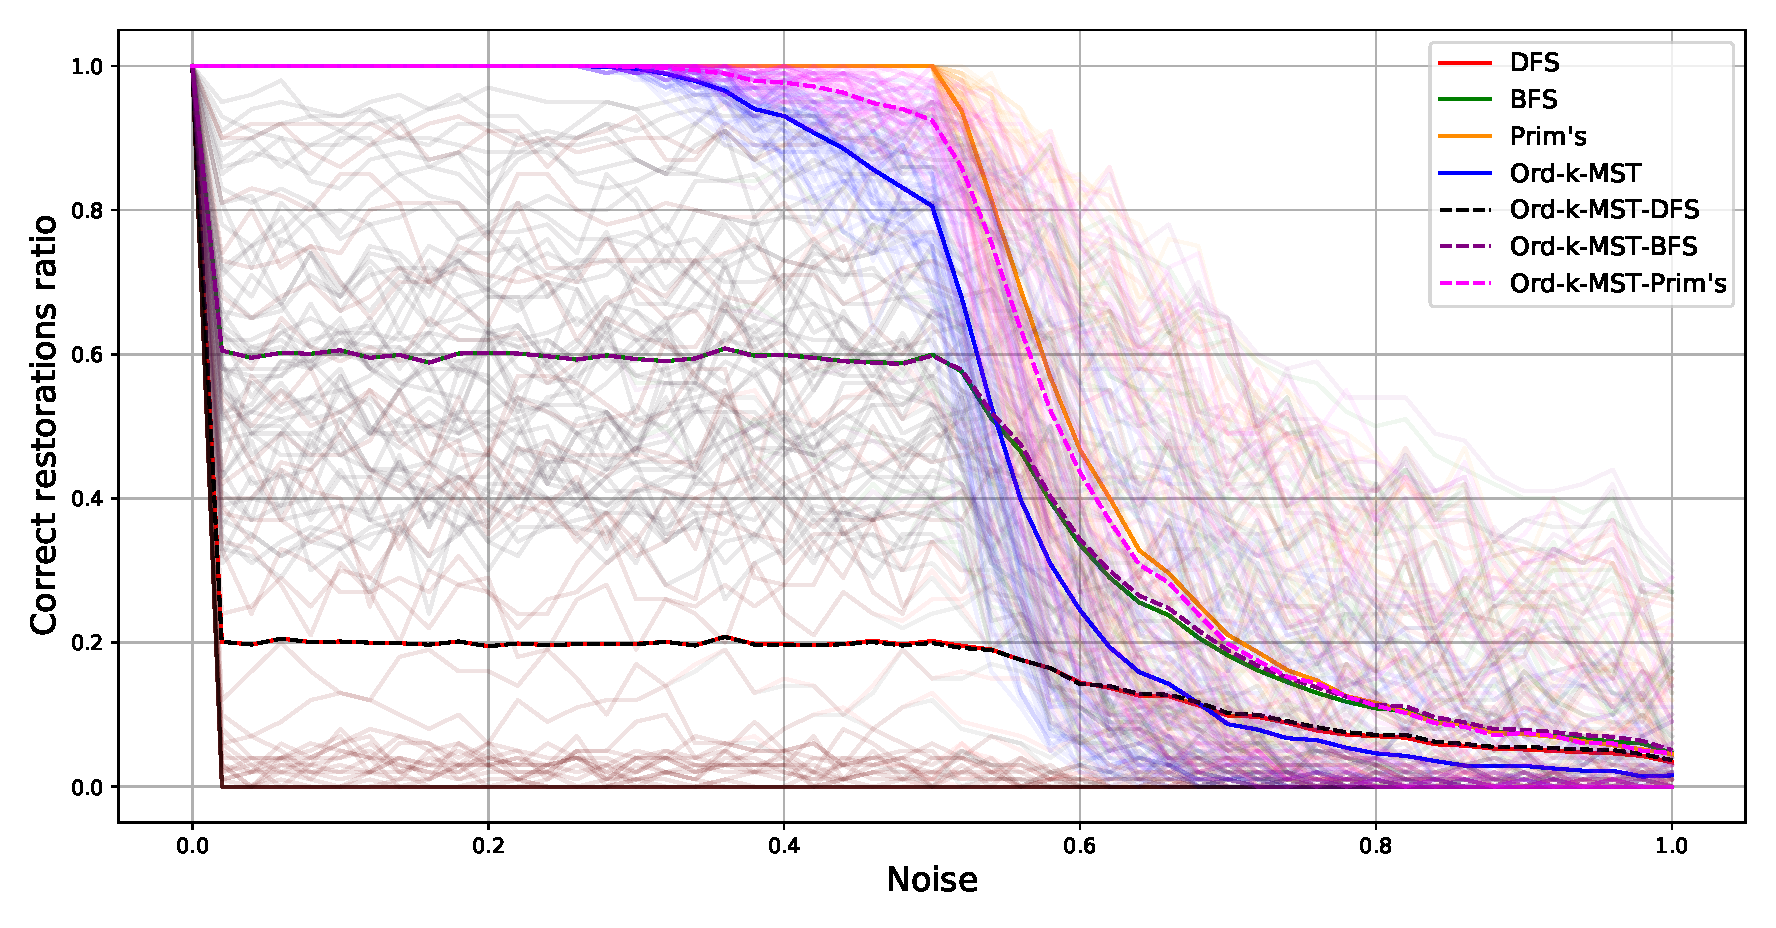
\includegraphics[scale=0.5]{./img/incor_algs_full_alpha006_maxarity_5_20.pdf}
    \caption{Ratio of correct restoration with different noise values. Arity $\in [5; 20]$, $k$-MST based algorithms use symmetric adjacency matrix.}
    \label{ris:5_20_arity_uniform_ord}
\end{figure}

\begin{minipage}[B]{0.49\textwidth}
    \centering
    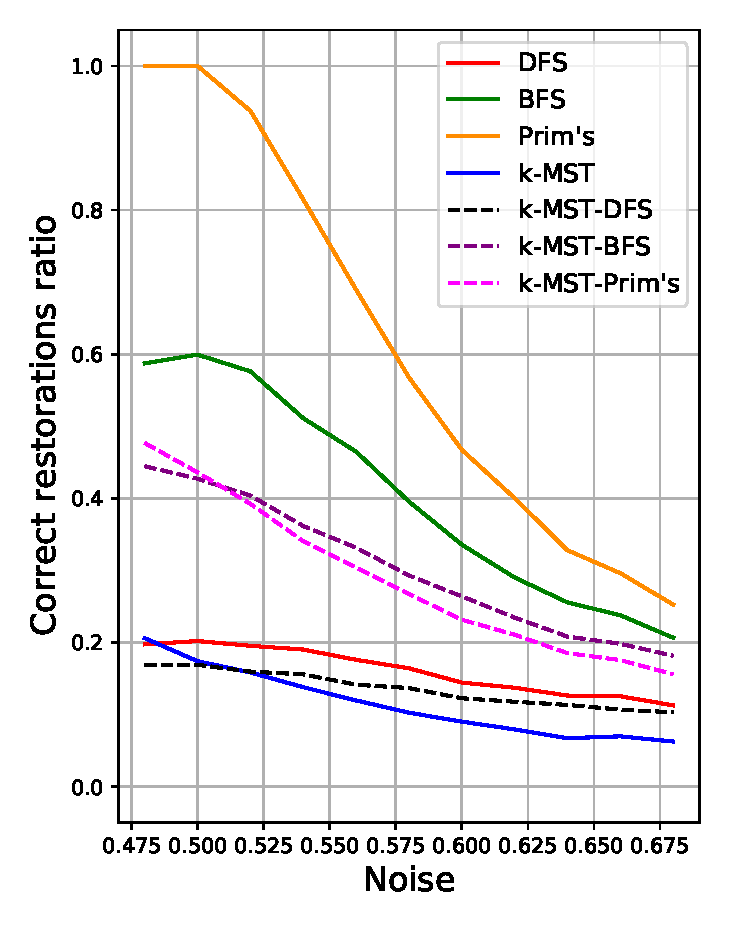
\includegraphics[width=0.7\textwidth]{img/main_algs_local_alpha000_maxarity_5_20.pdf}
    \captionof{figure}{Quality of the algorithms on the border; small arities; Uniform noise; unordered input}
    \label{ris:main_algs_local}
\end{minipage}
\hfill
\begin{minipage}[B]{0.49\textwidth}
        \centering
        \begin{tabular}{|c||c|c|c|c|c|}
            \hline
            $\text{Noise}$      &.50&.52&.54&.56&.58\\
            \hline
            \hline
            $\text{DFS}$                &.2  &.2 &.19 &.18 &.16\\
            \hline
            $\text{BFS}$                &.6  &.58 &.51 &.46 &.4\\
            \hline
            $\text{Prim's algorithm}$       &\textbf{1.0}  &\textbf{.94}&\textbf{.81}&\textbf{.69}&\textbf{.57}\\
            \hline
            $k\text{-MST}$          &.17  &.16 &.14 &.12 &.1\\
            \hline
            $k\text{-MST}$-$\text{DFS}$     &.17  &.16 &.16 &.14 &.14 \\
            \hline
            $k\text{-MST}$-$\text{BFS}$     &.43  &.4 &.36 &.33 &.29 \\
            \hline
            $k\text{-MST}$-Prim's   &.44  &.39 &.34 &.33 &.27 \\
            \hline
        \end{tabular}
        \captionof{table}{Quality with noise $\sim 0.5$}
        \label{table:main_algs_local}
\end{minipage}
The ordered versions of the $k$-MST based algorithms are illustrated on Fig. \ref{ris:incor_algs_full}. Prim's algorithm and $k$-MST show much closer restoration ratios. Algorithms based on $k$-MST deliver significantly better results. Algorithms based on $k$-MST and using BFS, DFS or Prim's algorithm to restore the original matrix show achieve results close to the sole results of BFS, DFS and Prim's algorithm accordingly. 

\begin{minipage}[B]{0.49\textwidth}
        \centering
        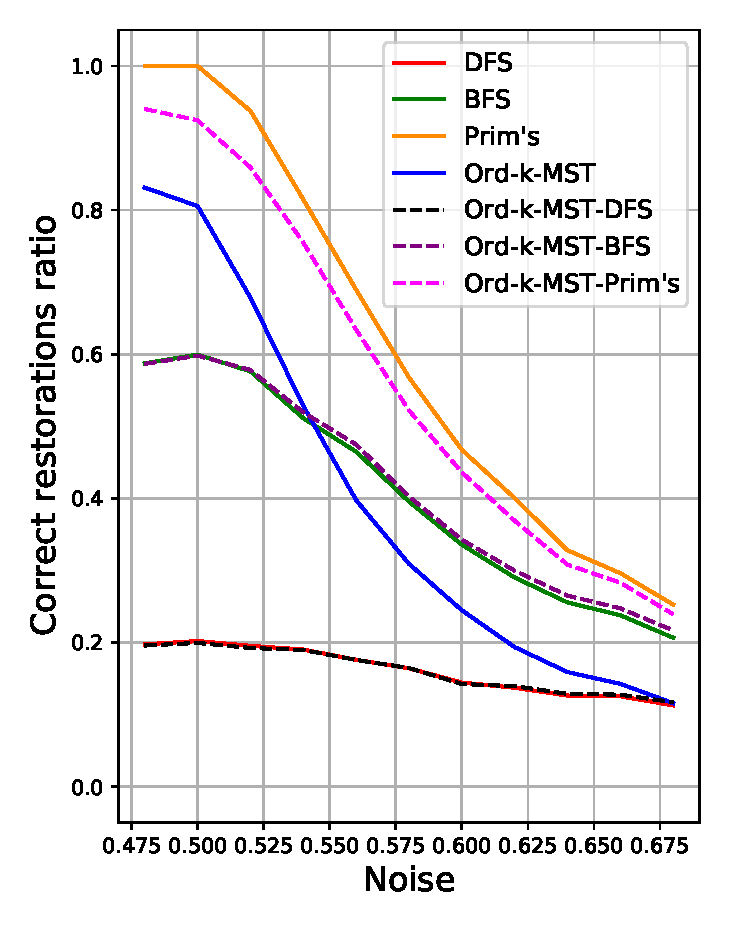
\includegraphics[scale=0.5]{img/incor_algs_local_alpha000_maxarity_5_20.pdf}
        \captionof{figure}{Ratio of correct restoration with different noise values. Arity $\in [5; 20]$, $k$-MST based algorithms use original adjacency matrix.}
        \label{ris:incor_algs_local}
\end{minipage}
\hfill
\begin{minipage}[B]{0.49\textwidth}
        \centering
        \begin{tabular}{|c||c|c|c|c|c|}
            \hline
            Noise       &.50 &.52&.54&.56&.58\\
            \hline
            \hline
            DFS                 &.2  &.2 &.19 &.18 &.16\\
            \hline
            BFS                 &.6  &.58 &.51 &.46 &.4\\
            \hline
            Prim's algorithm &\textbf{1.0}  &\textbf{.94} &\textbf{.81} &\textbf{.69} &\textbf{.57} \\
            \hline
            Ord-$k$-MST         &.81  &.68 &.53 &.4 &.31\\
            \hline
            Ord-$k$-MST-DFS     &.2  &.19 &.19 &.18 &.16\\
            \hline
            Ord-$k$-MST-BFS     &.6  &.58 &.52 &.47 &.4 \\
            \hline
            Ord-$k$-MST-Prim's  &.92  &.86 &.76 &.63 &.52 \\
            \hline
        \end{tabular}
        \captionof{table}{Ratio of correct restorations with noise $\sim 0.5$}
        \label{table:incor_algs_local}
\end{minipage}

Fig. \ref{ris:incor_algs_local} and Table \ref{table:incor_algs_local} illustrate the algorithms performance with noise close to $0.5$.

\begin{figure}
    \centering
    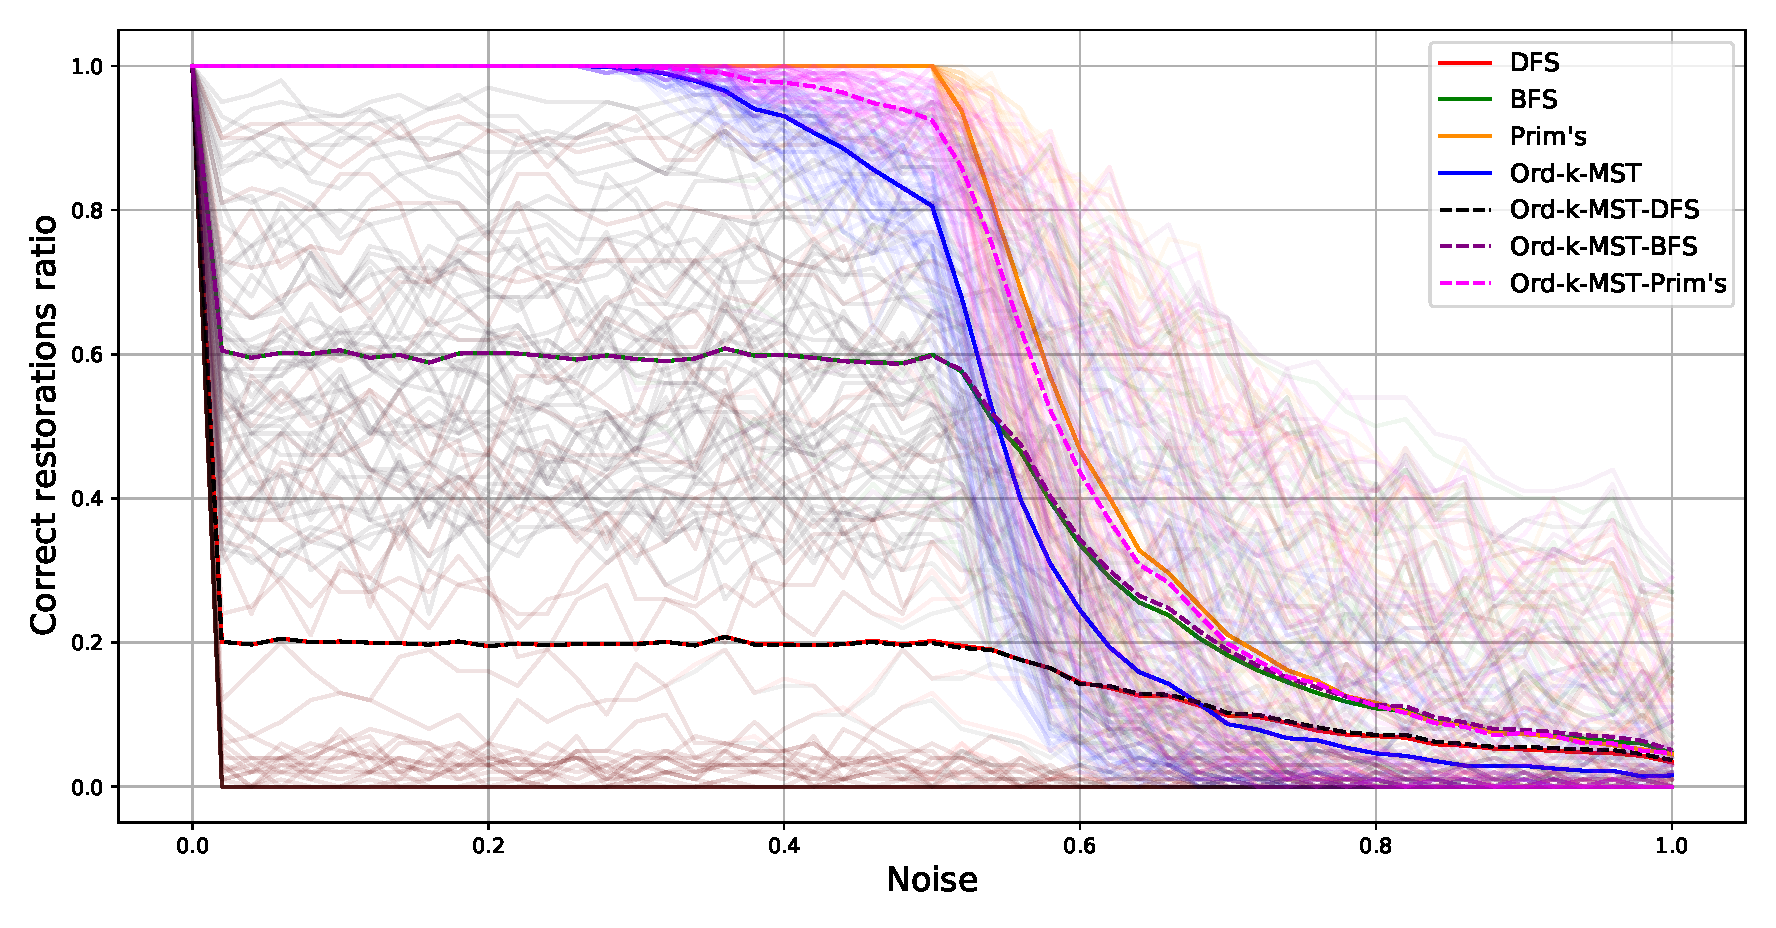
\includegraphics[scale=0.5]{./img/incor_algs_full_alpha006_maxarity_5_20.pdf}
    \caption{Quality of the algorithms on the border; arities $\in [5; 20$; Uniform noise; ordered input}
    \label{ris:incor_algs_full}
\end{figure}

Table \ref{fig:time} illustrates the time complexity of the described algorithms. The measurements were performed using $51\cdot 50\cdot 20\cdot5 \approx 250000$ matrix restorations.

\begin{figure}
    \centering
    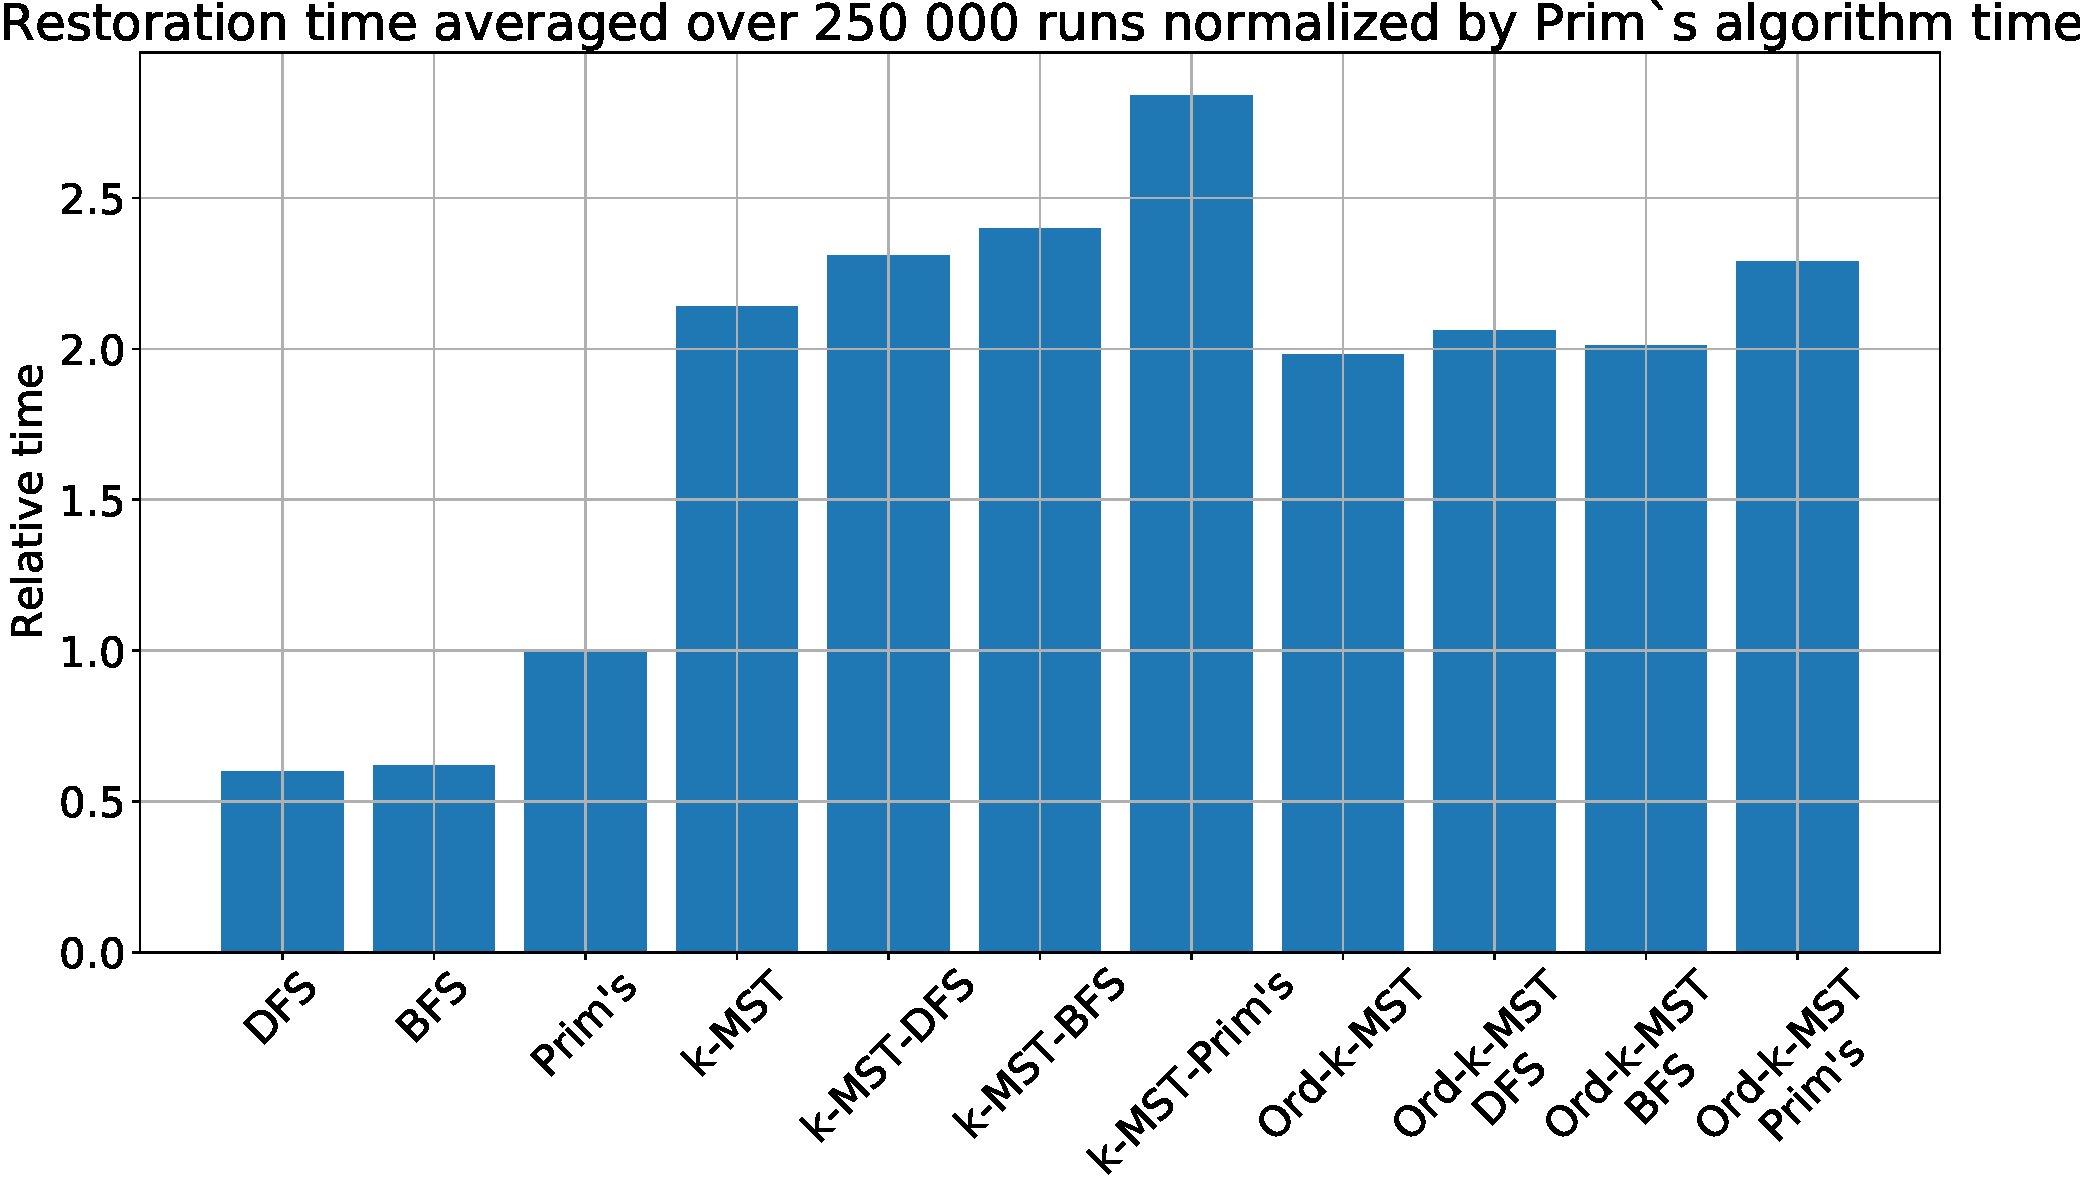
\includegraphics[scale=0.35]{./img/timing_comparison.pdf}
    \caption{Time comparison. All scores are normalized by Prim's algorithm elapsed time.}
    \label{fig:time}
\end{figure}
% \begin{table}
%     \begin{center}
        
%     \begin{tabular}{|r|r|r|r|r|r|r|r|}
%     \hline
%       Algorithm & DFS &   BFS &   Prim's &   $k$-MST &   $k$-MST-DFS & $k$-MST-BFS & $k$-MST-Prim's  \\
%     \hline
      
%       Relative time & 0.72 &  0.76 &        1 &      2.25 &          2.42 &          2.48 & 2.79  \\
%     \hline
%     \end{tabular}
%     \end{center}
% \end{table}
% \begin{table}
%     \begin{center}
%     \begin{tabular}{|r|r|r|r|r|}
%     \hline
%       Algorithm &      Ord-$k$-MST &   Ord-$k$-MST-DFS &   Ord-$k$-MST-BFS &   Ord-$k$-MST-Prim's \\
%     \hline
%       Relative time &           1.9  &              1.96 &              1.99 &                 2.22 \\
%     \hline
%     \end{tabular}
%     \end{center}
%   \label{table:time}
%   \caption{Time comparison. All scores are normalized by Prim's algorithm elapsed time.}
% \end{table}

\section{Conclusion}

This paper compares different approaches to symbolic regression problem based on restoration of the superposition matrix. The approach based on Prim's algorithm delivers the most accurate results and is the most resistant to small noise in data. 

The proposed algorithm delivers accurate results, but is more prone to noise in the superposition matrix.

Approaches based on BFS and DFS are unable to restore the original superposition if noise is present. PCST algorithm with BFS used for superposition matrix restoration shows mediocre results.

\begin{acknowledgments}
The reported study was funded by RFBR according to the research projects 20-37-90050, 19-07-01155 and NTI project 13/1251/2018.
\end{acknowledgments}

%
% The Bibliography
%

\begin{thebibliography}{99}
\bibitem{davis1991handbook}
\refitem{book}
L.~D.~Davis, \emph{Handbook Of Genetic Algorithms} (Van Nostrand Reinhold; 1st Edition, 1991).

\bibitem{koza1994genetic}
\refitem{article}
J.~R.~Koza \textquotedblleft "Genetic programming as a means for programming computers by natural selection",\textquotedblright Statistics and computing 4 (2) 87--112 (1994).
  
\bibitem{searson2010gptips}
\refitem{article}
D.~P.~Searson, D.~E.~Leahy, M.~J.~Willis, \textquotedblleft "GPTIPS: an open source genetic program- ming toolbox for multigene symbolic regression",\textquotedblright Proceedings of the International multiconference of engineers and computer scientists, 1, 77--80 (2010).

\bibitem{searson2015gptips}
\refitem{article}
D.~P.~Searson, \textquotedblleft GPTIPS 2: an open-source software platform for symbolic data mining,\textquotedblright Handbook of genetic programming applications, 551--573 (2016).

\bibitem{evolving2002}
\refitem{article}
K.~O.~Stanley, R.~Miikkulainen, \textquotedblleft Evolving neural networks through augmenting topologies,\textquotedblright Evolutionary computation 10 (2), 99--127 (2002).

\bibitem{wann2019}
\refitem{article}
A.~Gaier, D.~Ha, \textquotedblleft Weight Agnostic Neural Networks,\textquotedblright Advances in Neural Information Processing Systems 32, 5364--5378 (2019).

\bibitem{Bochkarev2017}
\refitem{article}
A.~M.~Bochkarev, I.~L.~Sofronov, V.~V.~Strijov, \textquotedblleft Generation of expertly-interpreted models for prediction of core permeability,\textquotedblright Systems and Means of Informatics 27 (3), 74--87 (2017).

\bibitem{lozovanu1993minimal}
\refitem{article}
D.~Lozovanu, A.~Zelikovsky, \textquotedblleft Minimal and bounded tree problems,\textquotedblright ezele Congre- sului XVIII al Academiei Romano-Americane,  25--26 (1993).

\bibitem{ravi1996spanning}
\refitem{article}
R.~Ravi, R.~Sundaram, M.~V.~Marathe et al., \textquotedblleft Spanning trees ~--- short or small,\textquotedblright SIAM Journal on Discrete Mathematics 9 (2), 178--200 (2015).

\bibitem{Chudak2004}
\refitem{article}
F.~A.~Chudak, T.~Roughgarden, D.~P.~Williamson, \textquotedblleft Approximate k-MSTs and k- Steiner trees via the primal-dual method and Lagrangean relaxation,\textquotedblright Mathematical Programming, 100 (2) 411--421 (2004).

\bibitem{awerbuch1998new}
\refitem{article}
 B.~Awerbuch, Y.~Azar, A.~Blum, S.~Vempala, \textquotedblleft New approximation guarantees for minimum-weight k-trees and prize-collecting salesmen,\textquotedblright SIAM Journal on computing, 28 (1), 254--262 (1998).

\bibitem{Arora2006}
\refitem{article}
 S.~Arora, G.~A.~Karakostas, \textquotedblleft 2 + $\varepsilon$ approximation algorithm for the k-MST problem,\textquotedblright Mathematical Programming, 107 (3), 491--504, (2006).

\bibitem{goemans1995general}
\refitem{article}
 M.~X.~Goemans, D.~P.~Williamson, \textquotedblleft A general approximation technique for constrained forest problems,\textquotedblright SIAM Journal on Computing, 24 (2), 296--317 (1995).

\bibitem{hegde2014fast}
\refitem{article}
 C.~Hegde, P.~Indyk, L.~Schmidt, \textquotedblleft A fast, adaptive variant of the Goemans-Williamson scheme for the prize-collecting Steiner tree problem,\textquotedblright Workshop of the 11th DIMACS Implementation Challenge, (2014).

\bibitem{pcstfast_alg}
\refitem{url}
\url{https://github.com/fraenkel-lab/pcst_fast}
 
\bibitem{Ras2017}
\refitem{article}
 C.~Ras, K.~Swanepoel, D.~A.~Thomas, \textquotedblleft Approximate Euclidean Steiner Trees,\textquotedblright  Journal of Optimization Theory and Applications, 172 (3), 845--873 (2017).

% \bibitem{hegde2014fast}
% \refitem{article}
%  R.~B.~Cole, R.~Hariharan, M.~Lewenstein, E.~Porat, \textquotedblleft A faster implementation of the Goemans-Williamson clustering algorithm,\textquotedblright SODA, (2017).

% \bibitem{pcstfast_alg}
% \refitem{url}
% \url{https://gitlab.com/Polkut/PCST_superposition_tree_reconstruction}

\end{thebibliography}

\newpage

\section{Supplementary materials}

Theorem 1 \begin{proof}
    Assume there is empty set $\emptyset\not=S\subset V,$ such that $\sum\limits_{e\in \delta(S)}x_e < f(S)$.
    Then $f(S) = 1$. For every connected component $C_1,\ldots,C_m$ from $(V,F')$ one of the following equations stand:
    $C_i\subseteq S$ or $C_i\cap S = \emptyset$ (according to $\sum\limits_{e\in \delta(S)}x_e=0$). 
    According to Lemma \ref{lem2} and disjunctive property, $f(S) = f\lp\bigcup\limits_{j}C_{i_j}\rp = 0$, which is contrary to the original assumption $f(S) = 1$.
\end{proof}

Theorem 2 \begin{proof}
    Recall the following inequality:
    $$
    Z_{LP}^{\ast}\leqslant \sum\limits_{e\in F'}c_e \leqslant \lp 2 - \frac{2}{|A|}\rp Z_{\text{DRLP}}\leqslant 
    \lp 2 - \frac{2}{|A|}\rp Z_{LP}^{\ast}.
    $$
    \begin{itemize}
        \item The first part is correct according to the $Z_{LP}^{\ast}$ definition and the fact that $F'$ meets the constraints (according to Theorem \ref{theorem1}).
        \item The last part is correct because for the optimal solution $Z_{LP}^{\ast}$ of Problem \ref{ilp_cfp} the following inequality holds (due to the below constraints of the dual problem): $Z_{\text{DRLP}} =  \sum_{S\subset V}y_S \leqslant Z_{RLP}^{\ast}\leqslant Z_{LP}^{\ast}$.
        \item The middle part should be proven explicitly.
    \end{itemize}
    
    After the Algorithm \ref{alg_general} stops $c_e = \sum y_S$, so the following equation stands:
    $$\sum\limits_{e\in F'}c_e = \sum\limits_{e\in F'}\sum\limits_{S:e\in \delta(S)}y_S = \sum\limits_{S\subset V}y_S\cdot |F'\cap \delta(S)|.$$
    
    So the following inequality should will be proved by induction:
    $$\sum\limits_{e\in F'}c_e = \sum\limits_{S\subset V}y_S\cdot |F'\cap \delta(S)|\leqslant \lp 2 - \frac{2}{|A|}\rp Z_{\text{DRLP}}=\lp 2 - \frac{2}{|A|}\rp \sum\limits_{S\subset V}y_S.$$
    
    \textbf{Basis case:} On the first step of the algorithm $y_S = 0$.
    
    \textbf{Inductive step:} assume the induction hypothesis that for a particular step k, the inequality holds. On the $(k+1)$ step the left hand side is increased by $\varepsilon\sum\limits_{S\in\mathcal{C}_a}|F'\cap \delta(S)|$, where $\mathcal{C}_a$ stays for all active components and  $f(C)=1$. The right hand side will be increased by $\varepsilon\lp 2 - \frac{2}{|A|}\rp\cdot|\mathcal{C}_a|$. Let's focus on the following inequality: 
    $$
    \sum\limits_{S\in\mathcal{C}_a}|F'\cap \delta(S)|\leqslant\lp 2 - \frac{2}{|A|}\rp\cdot|\mathcal{C}_a|.
    $$
    Denote the number of edges starting in $S$ as $d(S) = |F'\cap \delta(S)|$. So
    $$
    \sum\limits_{S\in\mathcal{C}_a}d(S) = \sum\limits_{S\in\mathcal{C}}d(S) - \sum\limits_{S\in\mathcal{C}_i}d(S) \leqslant 2(|\mathcal{C}_a| + |\mathcal{C}_i| -1) - \sum\limits_{S\in\mathcal{C}_i}d(S),
    $$
    where $\mathcal{C} = \mathcal{C}_i\cup \mathcal{C}_a$. The last inequality holds because $F'$ defines a forest in the original graph. The last step is to prove that
    \begin{align}
    \sum\limits_{S\in\mathcal{C}_i}d(S)\geqslant 2|\mathcal{C}_i|,
    \label{no_inactive_leafs}
    \end{align}
    which implies
    $$
    \sum\limits_{S\in\mathcal{C}_a}d(S) \leqslant 2(|\mathcal{C}_a| + |\mathcal{C}_i| -1) - 2|\mathcal{C}_i| = 2\lp 1 - \frac{1}{|\mathcal{C}_a|}\rp\cdot|\mathcal{C}_a|\leqslant2\lp 1 - \frac{1}{|A|}\rp\cdot|\mathcal{C}_a|,
    $$
     which is correct because the number of clusters does not increase through time, or equivalently $|A| \geqslant |\mathcal{C}_a|$.
     
    The following lemma will prove the inequality $(\ref{no_inactive_leafs})$.
    \begin{lemma}
        Denote graph $H$ where every vertex is corresponding to one of the connected components $C\in \mathcal{C}$ on the fixed step of the algorithm. Edge $(v_1,v_2)$ is present if there exists an edge $\hat{e}$ of the original graph included in $F'$: $\hat{e} \in F'$ (so the graph $H$ is a forest). There are no leaf vertices within $H$ such that correspond to inactive vertices in the original graph.
    \label{lemma_small}      
    \end{lemma}
    \begin{proof}
         Recall that lone inactive vertices are ignored due to the zero power of every inactive vertex, so they all can be subtracted in the inequality $\sum\limits_{S\in\mathcal{C}}d(S) \leqslant 2(|\mathcal{C}_a| + |\mathcal{C}_i| -1)$.
         
         Assume there is a leaf vertex $v\in V(H)$ connected with edge $e$. This vertex corresponds to the inactive set $C_v\in\mathcal{C}$. This set $C_v$ is included in one of the connected components $N\in F$, where $F$ is the set of vertices before pruning. The fact that $v \in V(H)$ is a leaf implies that all edges connecting $C_v$ with other vertices from $N$ but the edge $e$ were excluded during pruning.
         
         If the edge $e$ is excluded from the component $N$ (which is a tree itself), the component splits into $N_1$ and $N_2$. Without loss of generality assume $C_v\subseteq N_1$. The edge $e$ was not pruned, so $f(N_1)=1$ or $f(N_2)=1$. Due to $f(N) = 0$, the only possible variant is $f(N_1) = f(N_2) = 1$. Other cases are contradictory to Lemma \ref{lem1}.
         
         Denote components $(C_v,C_1,\ldots,C_m)$ derived from $N_1$ if edges from $F'$ are used. For every component but $C_v$ $f(C_i)=0 \forall i \neq v$ (the edges were pruned). But $f(C_v)=0$ according to the original assumption. Hence $f(N_1) = f\lp\bigcup\limits_{i=1}^{m} C_i \cup C_v\rp = 0$ by symmetry, which is contradictory to $f(N_1) = 1$. So there are no leaf vertices in $H$ which correspond to inactive vertices in the original graph, hence power of every inactive vertex is greater or equal to two (or equal to zero, but such vertices do not affect the target inequality).
    \end{proof}

    According to the Lemma \ref{lemma_small} proves the inequality $(\ref{no_inactive_leafs})$, so the second part of the original statement is also correct.
\end{proof}
\end{document}
